\section{Photovoltaic Arrays}\label{photovoltaic-arrays}

The Photovoltaics module includes three different models referred to as ``Simple'', ``Equivalent One-Diode'' and ``Sandia'' and the choice will determine the mathematical models (and input data) used to determine the energy produced by solar/electric conversion panels. There is also a PVWatts generator which abstracts away specifying PV modules and array properties for a simpler input structure. The EnergyPlus photovoltaic array models are called one at a time at the HVAC system timestep along with other electrical generation components such as gas turbines and diesel engines.

All of the photovoltaic models with the exception of the PVWatts model share the same models for predicting incident solar radiation that are also used for the solar thermal calculations and are described in the section Climate, Sky and Solar/Shading Calculations. The PVWatts generator uses the same solar calculations as the SAM software or PVWatts web API. 

Note that some of the terminology used to discussed photovoltaics overlaps with terminology in software development and both may apply in these descriptions. The word \emph{module} may refer to a PV panel or to a C++ programming entity. \emph{Model} may refer to a manufacturers production model for a specific type of PV module or to a mathematical model used for engineering analysis. \emph{Array} may refer to a collection of PV modules wired together or to a mathematical variable with multiple elements.

The PV modules are assumed to always run when the total incident solar is greater than 0.3 Watts. If the incident solar is less than 0.3, then the modules produce no power.

PV arrays are managed by an electric load center. The load center is a ``load'' with respect to generating equipment but is a ``supply center'' for the rest of the building. PV arrays need to be connected to ElectricLoadCenter:Distribution objects that have a DC buss type.

\subsection{Simple Model}\label{simple-model}

The Generator:PV:Simple object describes about the simplest model for predicting photovoltaic energy production. In this model the user specifies the efficiency with which surfaces convert incident solar radiation to electricity. (In the other models this efficiency is determined as part of the model.)~ The full geometric model for solar radiation is used, including sky models, shading, and reflections, to determine the incident solar resource. The model accepts arbitrary conversion efficiencies and does not require actual production units be tested to obtain empirical performance coefficients. (The Energy+.idd sets the range of conversion efficiencies to be within {[}0..1{]}, but the user could alter the Energy+.idd to extend this range if desired.)

\subsubsection{Mathematical Description}\label{mathematical-description}

% table 89
\begin{longtable}[l]{p{1.2in}p{4.8in}}
\caption{Nomenclature for Simple Photovoltaic model \label{table:nomenclature-for-simple-photovoltaic-model}} \tabularnewline
\toprule 
Mathematical Variable & Description \tabularnewline
\midrule
\endfirsthead

\caption[]{Nomenclature for Simple Photovoltaic model} \tabularnewline
\toprule 
Mathematical Variable & Description \tabularnewline
\midrule
\endhead

P & Electrical power produced by photovoltaics (W) \tabularnewline
A\(_{surf}\) & Net area of surface~ (m\(^{2}\)) \tabularnewline
f\(_{activ}\) & Fraction of surface area with active solar cells \tabularnewline
G\(_{T}\) & Total solar radiation incident on PV array (W/m\(^{2}\)) \tabularnewline
$\eta$\(_{cell}\) & Module conversion efficiency \tabularnewline
$\eta$\(_{invert}\) & DC to AC conversion efficiency \tabularnewline
\bottomrule
\end{longtable}

The usable electrical power produced by a PV surface are calculated using:

\begin{equation}
P = {A_{surf}} \cdot {f_{activ}} \cdot {G_T} \cdot {\eta_{cell}} \cdot {\eta_{invert}}
\end{equation}

On the right hand side of this equation, only G\(_{T}\) is calculated by EnergyPlus and the rest are user inputs. Power levels are assumed constant over the timestep to arrive at energy production.

There are two modes that can be selected by the user that govern how the PV system is coupled to the building surfaces. If the integration mode is selected as `DECOUPLED' then no adjustments are made to account for energy extracted in the form of electricity. If the integration mode is selected as `INTEGRATED' then the energy extracted in the form of electricity is removed from surface heat transfer calculations using a sink term. This sink term is lagged from the previous timestep.

\subsection{Equivalent One-Diode Model}\label{equivalent-one-diode-model}

This model predicts the electrical performance of a photovoltaic (PV) array. This model is also known as the ``TRNSYS PV'' model.

Mathematically speaking, the EnergyPlus PV module employs equations for an empirical equivalent circuit model to predict the current-voltage characteristics of a single module. This circuit consists of a DC current source, diode, and either one or two resistors. The strength of the current source is dependent on solar radiation and the IV characteristics of the diode are temperature-dependent. The results for a single module equivalent circuit are extrapolated to predict the performance of a multi-module array.

The module employs a ``four-parameter'' equivalent circuit to model crystalline (both mono and poly) PV modules developed at the University of Wisconsin -- Madison. The values of these parameters cannot normally be obtained directly from manufacturers' catalogs. However, the PV module will automatically calculate them from commonly available data. The PV module also includes an optional incidence angle modifier correlation to calculate how the reflectance of the PV module surface varies with the angle of incidence of solar radiation.

The module determines PV current as a function of load voltage. Other OUTPUTS include current and voltage at the maximum power point along the IV curve, open-circuit voltage, short circuit current as well as electrical load met and unmet.

% table 90
\begin{longtable}[l]{p{1.2in}p{4.8in}}
\caption{General Nomenclature for the PV model \label{table:general-nomenclature-for-the-pv-model}} \tabularnewline
\toprule 
Mathematical variable & Description \tabularnewline
\midrule
\endfirsthead

\caption[]{General Nomenclature for the PV model} \tabularnewline
\toprule 
Mathematical variable & Description \tabularnewline
\midrule
\endhead

$\beta$ & Slope of PV array (degrees) \tabularnewline
$\gamma$ & Empirical PV curve-fitting parameter \tabularnewline
$\varepsilon$\(_{\gamma}\) & Semiconductor bandgap (eV) \tabularnewline
$\eta$\(_{c}\) & Module conversion efficiency \tabularnewline
$\mu$\(_{isc}\) & Temperature coefficient of short-circuit current (A/K) \tabularnewline
$\mu$\(_{voc}\) & Temperature coefficient of open-circuit voltage (V/K) \tabularnewline
$\theta$ & Angle of incidence for solar radiation (degrees) \tabularnewline
$\tau\alpha$ & Module transmittance-absorptance product \tabularnewline
$\tau\alpha$\(_{normal}\) & Module transmittance-absorptance product at normal incidence \tabularnewline
G\(_{T}\) & Total radiation incident on PV array \tabularnewline
G\(_{T,beam}\) & Beam component of incident radiation \tabularnewline
G\(_{T,diff}\) & Diffuse component of incident radiation \tabularnewline
G\(_{T,gnd}\) & Ground-reflected component of incident radiation \tabularnewline
G\(_{T,NOCT}\) & Incident radiation at NOCT conditions \tabularnewline
G\(_{T,ref}\) & Incident radiation at reference conditions \tabularnewline
I & Current \tabularnewline
I\(_{L}\) & Module photocurrent \tabularnewline
I\(_{L,ref}\) & Module photocurrent at reference conditions \tabularnewline
I\(_{o}\) & Diode reverse saturation current \tabularnewline
I\(_{o,ref}\) & Diode reverse saturation current at reference conditions \tabularnewline
I\(_{sc}\) & Short-circuit current \tabularnewline
I\(_{sc,ref}\) & Short-circuit current at reference conditions \tabularnewline
I\(_{mp}\) & Current at maximum power point along IV curve \tabularnewline
I\(_{mp,ref}\) & Current at maximum power point along IV curve, reference conditions \tabularnewline
IAM & Dimensionless incidence angle modifier \tabularnewline
K & Boltzmann constant (J/K) \tabularnewline
NP & Number of modules in parallel in array \tabularnewline
NS & Number of modules in series in array \tabularnewline
N\(_{s}\) & Number of individual cells in module \tabularnewline
P & PV output power \tabularnewline
P\(_{max}\) & PV output power at maximum power point along IV curve \tabularnewline
Q & Electron charge constant \tabularnewline
R\(_{s}\) & Module series resistance ($\Omega$) \tabularnewline
R\(_{sh}\) & Module shunt resistance ($\Omega$) \tabularnewline
T\(_{c}\)­ & Module temperature (K) \tabularnewline
T\(_{c,NOCT}\) & Module temperature at NOCT conditions (K) \tabularnewline
T\(_{c,ref}\) & Module temperature at reference conditions (K) \tabularnewline
U\(_{L}\) & Array thermal loss coefficient \tabularnewline
V & Voltage \tabularnewline
V\(_{mp}\) & Voltage at maximum power point along IV curve \tabularnewline
V\(_{mp,ref}\) & Voltage at maximum power point along IV curve, reference conditions \tabularnewline
V\(_{oc}\)­ & Open-circuit voltage \tabularnewline
V\(_{oc,ref}\) & Open-circuit voltage at reference conditions (V) \tabularnewline
\bottomrule
\end{longtable}

\subsubsection{Mathematical Description}\label{mathematical-description-1}

\paragraph{PV Section 1: Four-Parameter Model}\label{pv-section-1-four-parameter-model}

The four-parameter equivalent circuit model was developed largely by Townsend {[}1989{]} and is detailed by Duffie and Beckman {[}1991{]}. The model was first incorporated into a component for the TRNSYS simulation package by Eckstein {[}1990{]}. The EnergyPlus module employs the Eckstein model for crystalline PV modules, using it whenever the short-circuit IV slope is set to zero or a positive value as modified by Ulleberg {[}2000{]}. The four parameter model assumes that the slope of the IV curve is zero at the short-circuit condition:

\begin{equation}
{\left( {\frac{{dI}}{{dV}}} \right)_{v = 0}} = 0
\end{equation}

This is a reasonable approximation for crystalline modules. The ``four parameters'' in the model are \(I_{L,ref}\), \(I_{o,ref}\), \(\gamma\), and \(R_{s}\). These are empirical values that cannot be determined directly through physical measurement. The EnergyPlus model calculates these values from manufactures' catalog data as discussed in the following section on calculating these parameters.

The four-parameter equivalent circuit is shown in Figure~\ref{fig:equivalent-circuit-in-the-four-parameter}.

\begin{figure}[hbtp] % fig 339
\centering
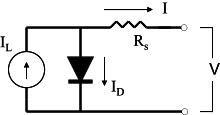
\includegraphics[width=0.9\textwidth, height=0.9\textheight, keepaspectratio=true]{media/image7592.svg.png}
\caption{Equivalent circuit in the four parameter model \protect \label{fig:equivalent-circuit-in-the-four-parameter}}
\end{figure}

\emph{V} is the load voltage and \emph{I} is the current flowing through the load and PV.

\textbf{Determining Performance under Operating Conditions}

The IV characteristics of a PV change with both insolation and temperature. The PV model employs these environmental conditions along with the four module constants \(I_{L,ref}\), \(I_{o,ref}\), \(\gamma\), and \(R_{s}\) to generate an IV curve at each timestep.

The current-voltage equation of circuit shown in Figure~\ref{fig:equivalent-circuit-in-the-four-parameter} is as follows:

\begin{equation}
I = {I_L} - {I_o}\left[ {\exp \left( {\frac{q}{{\gamma k{T_c}}}\left( {V + I{R_s}} \right)} \right) - 1} \right]
\label{eq:ElecLoadI869}
\end{equation}

where \(R_{s}\) and \(\gamma\) are constants. The photocurrent \(I_{L}\) depends linearly on incident radiation:

\begin{equation}
{I_L} = {I_{L,ref}}\frac{{{G_T}}}{{{G_{T,ref}}}}
\label{eq:ElecLoadIL870}
\end{equation}

The reference insolation \(G_{ref}\) is nearly always defined as 1000 W/m\(^{2}\). The diode reverse saturation current \(I_{o}\) is a temperature dependent quantity:

\begin{equation}
\frac{{{I_o}}}{{{I_{o,ref}}}} = {\left( {\frac{{{T_c}}}{{{T_{c,ref}}}}} \right)^3}
\label{eq:ElecLoadIoOverIoref871}
\end{equation}

Equation~\ref{eq:ElecLoadI869} gives the current implicitly as a function of voltage. Once \(I_{o}\) and \(I_{L}\) are found from Equations~\ref{eq:ElecLoadIL870} and~\ref{eq:ElecLoadIoOverIoref871}, Newton's method is employed to calculate the PV current. In addition, an iterative search routine finds the current (\(I_{mp}\)) and voltage (\(V_{mp}\)) at the point of maximum power along the IV curve.

\textbf{Calculating \(I_{L,ref}\), \(I_{o,ref}\), \(\gamma\), and \(R_{s}\)}

The Idf specification for the PV model include several values which must be read from manufacturers' PV module catalogs. The manufactures' values are used to determine the equivalent circuit characteristics \(I_{L,ref}\), \(I_{o,ref}\), \(\gamma\), and \(R_{s}\). These characteristics define an equivalent circuit that is employed to find the PV performance at each timestep, as described previously. This section describes the algebra and calculation algorithms used to solve for the four equivalent circuit characteristics.

Three of these values, \(I_{L,ref}\), \(I_{o,ref}\), and \(\gamma\) may be isolated algebraically. The first step is to substitute the current and voltage into Equation~\ref{eq:ElecLoadI869} at the open-circuit, short circuit, and maximum power conditions:

\begin{equation}
0 = {I_{L,ref}} - {I_{o,ref}}\left[ {\exp \left( {\frac{q}{{\gamma k{T_{c,ref}}}}{V_{oc,ref}}} \right) - 1} \right] - \frac{{{V_{oc,ref}}}}{{{R_{sh}}}}
\end{equation}

\begin{equation}
{I_{sc,ref}} = {I_{L,ref}} - {I_{o,ref}}\left[ {\exp \left( {\frac{{q{I_{sc,ref}}{R_s}}}{{\gamma k{T_{c,ref}}}}} \right) - 1} \right] - \frac{{{I_{sc,ref}}{R_s}}}{{{R_{sh}}}}
\end{equation}

\begin{equation}
{I_{mp,ref}} = {I_{L,ref}} - {I_{o,ref}}\left[ {\exp \left( {\frac{q}{{\gamma k{T_{c,ref}}}}\left( {{V_{mp,ref}} + {I_{mp,ref}}{R_s}} \right)} \right) - 1} \right] - \frac{{{V_{mp,ref}} + {I_{mp,ref}}{R_s}}}{{{R_{sh}}}}
\end{equation}

In each case the ``-1'' term is/may be dropped to simplify the algebra. This approximation has little influence on the right side of the equations since because the magnitude of \emph{I\(_{o}\)} is very small, generally on the order of 10\(^{-6}\) A. Some rearrangement then yields the following three expressions which isolate \(I_{L,ref}\), \(I_{o,ref}\), and \(\gamma\):

\begin{equation}
{I_{L,ref}} \approx {I_{sc,ref}}
\label{eq:ElecLoadILref875}
\end{equation}

\begin{equation}
\gamma  = \frac{{q\left( {{V_{mp,ref}} - {V_{oc,ref}} + I_{mp,ref}^{}{R_s}} \right)}}{{k{T_{c,ref}}\ln \left( {1 - \frac{{{I_{mp,ref}}}}{{{I_{sc,ref}}}}} \right)}}
\label{eq:ElecLoadGamma876}
\end{equation}

\begin{equation}
{I_{o,ref}} = \frac{{{I_{sc,ref}}}}{{\exp \left( {\frac{{q{V_{oc,ref}}}}{{\gamma k{T_{c,ref}}}}} \right)}}
\label{eq:ElecLoadIoref877}
\end{equation}

At this point an additional equation is needed in order to determine the last unknown parameter. Taking the analytical derivative of voltage with respect to temperature at the reference open-circuit condition derives the fourth equation. This analytical value is matched to the open-circuit temperature coefficient, a catalog specification:

\begin{equation}
\frac{{\partial {V_{oc}}}}{{\partial {T_c}}} = {\mu_{voc}} = \frac{{\gamma k}}{q}\left[ {\ln \left( {\frac{{{I_{sc,ref}}}}{{{I_{o,ref}}}}} \right) + \frac{{{T_c}\mu_{isc}^{}}}{{{I_{sc,ref}}}} - \left( {3 + \frac{{q\varepsilon }}{{Ak{T_{c,ref}}}}} \right)} \right]
\label{eq:ElecLoaddVocdTc878}
\end{equation}

where:

\begin{equation}
A = \frac{\gamma }{{{N_s}}}
\end{equation}

The ``TRNSYS PV model'' uses an iterative search routine in these four equations to calculate the equivalent circuit characteristics. The first step is to set upper and lower bounds for the series resistance parameter \emph{R\(_{s}\)}:~ physical constraints require the \(R_{s}\) value to lie between 0 and the value such that \(\gamma\) = \(N_{s}\). The initial guess for \(R_{s}\) is midway between these bounds. \(\gamma\) and \(I_{o,ref}\) are found from Equations~\ref{eq:ElecLoadGamma876} and~\ref{eq:ElecLoadIoref877}, while Equation~\ref{eq:ElecLoadILref875} gives a trivial solution for \(I_{L,ref}\).~ The model then employs Equation~\ref{eq:ElecLoaddVocdTc878} to compare the analytical and catalog values for \(m_{voc}\). When all other variables are held constant, the analytical value for \(m_{voc}\) increases monotonically with series resistance (Townsend 1989). If the analytical voltage coefficient is less than the catalog value, the lower bound for \(R_{s}\) is reset to the present guess value. Likewise, the upper bound is set to the current value if the calculated \(m_{voc}\) is too large. After resetting the upper or lower bound for \(R_{s}\), a new guess value is found by averaging the bounds. This procedure repeats until \(R_{s}\) and \(\gamma\) converge. Note that for \(I_{L,ref}\), \(I_{o,ref,}\), \(\gamma\), and \(R_{s}\) are assumed to be constant and are calculated only on the first call in the simulation. Alternatively, the user may enter a known series resistance by entering a \textbf{positive} value in the IDF. In this case the iterative routine described above is skipped and Equations~\ref{eq:ElecLoadILref875},~\ref{eq:ElecLoadGamma876}, and~\ref{eq:ElecLoadIoref877} find \(I_{L,ref}\), \(I_{o,ref,}\), and \(\gamma\) directly from the given value of \(R_{s}\).

\paragraph{PV Section 2 : Module Operating Temperature}\label{pv-section-2-module-operating-temperature}

The PV model uses one of five methods for determining cell temperature data. The cell temperature of a PV module is important because the hotter the temperature of the panel, the lower its electrical output. The cell temperature calculation method is chosen by the user in the EnergyPlus IDF file through a parameter choice in the IDD entry called Integration and Cell Temperature Mode.

If the value of this parameter is ``\textbf{Decoupled NOCT Conditions}'' then the cell temperature of the PV is modeled using the method from the Duffie and Beckman (1991) for estimating cell temperature. This is based upon the standard NOCT (Nominal Operating Cell Temperature) measurements to compute the module temperature \(T_c\) at each timestep. The NOCT temperature (\(T_c\),NOCT) is the operating temperature of the module with a wind speed of 1 m/s, no electrical load, and a certain specified insolation and ambient temperature {[}Beckman and Duffie, 1991{]}. The values for insolation GT,NOCT ~and ambient temperature \(T_{a,NOCT}\) are usually 800 W/m\(^{2}\) and 20\(^{\circ}\)C. \(\eta_{c}\) is the convesion efficiency of the module, which varies with ambient conditions. \({\tau \alpha}\) is a user-defined constant.

The equation is:

\begin{equation}
  T_c = T_a + \frac{1-\frac{\eta_c}{\tau \alpha}}{G_T \tau\alpha/U_L}
\end{equation}

If the user specifies the ``\textbf{Decoupled Ulleberg Dynamic''} mode for calculating cell temperature, then a method developed by Ulleberg is used:

\begin{equation}
{\left. {{T_{cell}}} \right|_t} = {T_{ambient}} + \left( {{{\left. {{T_{cell}}} \right|}_{t - 1}} - {T_{ambient}}} \right)*{e^{\frac{{ - UL}}{{Cap}}\Delta t}}
\end{equation}

In other words, the cell temperature is a function of the privious cell temperature and the thermal capacity of the PV module material.

If the user specifies ``\textbf{Integrated Surface Outside Face''} for this parameter, then the temperature result from EnergyPlus's modeling of surfaces is used for the cell temperature. Also the energy exported from the surface as electricity becomes a sink in the internal source modeling for the heat transfer surface.

If the user specifies ``\textbf{Integrated Transpired Collector''} for this parameter, then the temperature result for the unglazed transpired collector surfaces is used for the cell temperature. Also the energy exported from the collector surface as electricity is deprecated using a source term in the collector's temperature modeling.

If the user specifies ``\textbf{Integrated Exterior Vented Cavity''} for this parameter, then the temperature result for the exterior cavity is used for the cell temperature. Also the energy exported from the baffle surface as electricity is deprecated using a source term in the baffle's temperature modeling.

\paragraph{PV Section 3 : Multi-Array Modules}\label{pv-section-3-multi-array-modules}

The electrical calculations discussed in the sections above deal only with a single module. The EnergyPlus PV component may be used to simulate arrays with any number of modules. The IDF defines the number of modules in series (NS) and modules in parallel (NP) for the entire array. The total number of modules in the array is the product of NS and NP. When simulating a single module only, both NS and NP are set to 1. The single-module values for all currents and voltages discussed in PV Section 1 are multiplied by NP or NS to find values for the entire array. This approach neglects module mismatch losses.

With the above equations, and the assumption that the panels operate at the maximum power point, it is a direct calculation to determine DC power production. The performance of an array of identical modules is assumed to be linear with the number of modules in series and parallel. The inverter efficiency is applied linearly to derate the energy production. The inverter capacity forms a limit for power production from a PV generator. A `load' is passed the PV array acting as a generator and various trivial calculations compare PV production to this load. If the PV array is associated with a surface that is associated with a zone, then if the zone has any multipliers associated with it, electricity production will be multiplied accordingly.

\subsubsection{References}\label{references-035}

Duffie, John A. and William A. Beckman. 1991. \emph{Solar Engineering of Thermal Processes}. New York: John Wiley \& Sons, Inc..

Eckstein, Jürgen Helmut. 1990. \emph{Detailed Modeling of Photovoltaic Components}. M. S. Thesis -- Solar Energy Laboratory, University of Wisconsin, Madison: 1990.

Ulleberg, Øystein. \emph{HYDROGEMS Component Library for TRNSYS 15 User Manual}, Institute for Energy Technology, Kjeller, Norway \emph{~}

\subsection{Sandia Photovoltaic Performance Model}\label{sandia-photovoltaic-performance-model}

The third model available in EnergyPlus for predicting the electricity generated by photovoltaics is referred to as the Sandia model. This model is based on work done at Sandia National Lab, Albuquerque, NM by David King -- with the help of many others. The model consists of a series of empirical relationships with coefficients that are derived from actual testing. Once the coefficients for a particular module are available, it is straightforward matter to use the model equations to calculate five select points on the current-voltage curve.

The C++ implementation in EnergyPlus is also based on work done by Greg Barker (2003) for the National Renewable Energy Lab who implemented the Sandia model in FORTRAN77 as a custom type (Type101) for the TRNSYS computer program.

There are several climate and solar orientation inputs to the model that are managed elsewhere in EnergyPlus including: incident beam solar, incident diffuse solar, incidence angle of beam solar, solar zenith Angle, outdoor drybulb, wind speed, and elevation.

\subsubsection{Mathematical Description}\label{mathematical-description-2}

This section presents the mathematical description of the Sandia model from a draft report by King et, al. (2003). The core of the model predicts the performance of a single PV module. The following nomenclature and equations summarize the Sandia model.

% table 91
\begin{longtable}[c]{p{1.2in}p{4.8in}}
\caption{Nomenclature for Sandia PV model \label{table:nomenclature-for-sandia-pv-model}} \tabularnewline
\toprule 
Mathematical variable & Description \tabularnewline
\midrule
\endfirsthead

\caption[]{Nomenclature for Sandia PV model} \tabularnewline
\toprule 
Mathematical variable & Description \tabularnewline
\midrule
\endhead

I\(_{sc}\) & Short-circuit current (A) \tabularnewline
I\(_{mp}\) & Current at the maximum-power point (A) \tabularnewline
I\(_{x}\) & Current at module V = 0.5 V\(_{oc}\), defines 4th point on I-V curve \tabularnewline
I\(_{xx}\) & Current at module V = 0.5 (V\(_{oc}\) + V\(_{mp}\)), defines a 5th point on the I-V curve \tabularnewline
V\(_{oc}\) & Open-circuit voltage (V) \tabularnewline
V\(_{mp}\) & Voltage at maximum-power point (V) \tabularnewline
P\(_{mp}\) & Power at maximum-power point (W) \tabularnewline
fd & Fraction of diffuse irradiance used by module \tabularnewline
N\(_{s}\) & Number of cells in series in a module’s cell-string \tabularnewline
N\(_{p}\) & Number of cell-strings in parallel in module \tabularnewline
k & Boltzmann’s constant, 1.38066E-23 (J/K) \tabularnewline
q & Elementary charge, 1.60218E-19 (coulomb) \tabularnewline
T\(_{c}\) & Cell temperature inside module (\(^{\circ}\)C) \tabularnewline
$\delta$(T\(_{c}\)) & ‘Thermal voltage’ per cell at temperature T\(_{c}\), approximately 1 volt for a typical 26-cell crystalline silicon module \tabularnewline
E\(_{e}\) & ‘Effective’ solar irradiance \tabularnewline
E\(_{b}\) & Beam solar irradiance \tabularnewline
E\(_{diff}\) & Diffuse solar irradiance \tabularnewline
C\(_{0}\), C\(_{1}\) & Empirical coefficients relating I\(_{mp}\) to E\(_{e}\), C\(_{0}\) + C\(_{1}\) = 1 (both dimensionless) \tabularnewline
C\(_{2}\), C\(_{3}\) & Empirical coefficients relating V\(_{mp}\) to E\(_{e}\) (C\(_{2}\) dimensionless, C\(_{3}\) is 1/V) \tabularnewline
C\(_{4}\), C\(_{5}\) & Empirical coefficients relating I\(_{x}\) to E\(_{e}\), C\(_{4}\) + C\(_{5}\) = 1 (both dimensionless) \tabularnewline
C\(_{6}\), C\(_{7}\) & Empirical coefficients relating I\(_{xx}\) to E\(_{e}\) C\(_{6}\) + C\(_{7}\) = 1 (both dimensionless) \tabularnewline
n & Empirically determined ‘diode factor’ for individual cells \tabularnewline
AMa & Absolute Air Mas \tabularnewline
AOI & Solar angle-of-incidence (degrees) from normal \tabularnewline
f\(_{1}\)(AM\(_{a}\)) & Empirical polynomial function used to relate short-circuit current to the solar spectrum via air mass \tabularnewline
f\(_{2}\)(AOI) & Empirical polynomial function used to relate short-circuit current to the solar angle-of-incidence \tabularnewline
a\(_{0}\), a\(_{1}\), a\(_{2}\), a\(_{3}\), a\(_{4}\) & Empirical coefficients for f\(_{1}\)(AM\(_{a}\)) polynomial \tabularnewline
b\(_{0}\), b\(_{1}\), b\(_{2}\), b\(_{3}\), b\(_{4}\),b\(_{5}\),b\(_{6}\) & Empirical coefficients for f\(_{2}\)(AOI) polynomial \tabularnewline
T\(_{o}\) & Reference cell temperature for rating, typically fixed at 25\(^{\circ}\)C \tabularnewline
I\(_{sco}\) & Short circuit current at reference conditions \tabularnewline
I\(_{mpo}\) & Max power point current at reference conditions \tabularnewline
V\(_{mpo}\) & Voltage at max power at reference conditions \tabularnewline
V\(_{oco}\) & Open circuit voltage at reference conditions \tabularnewline
I\(_{xo}\) & Current at V = 0.5 Voc and at reference conditions \tabularnewline
I\(_{xxo}\) & Current at V = 0.5 (Vmp + Voc) and at reference conditions \tabularnewline
$\alpha$\(_{Isc}\) & Normalized temperature coefficient for I\(_{sc}\) (1/\(^{\circ}\)C) \tabularnewline
$\alpha$\(_{Imp}\) & Normalized temperature coefficient for I\(_{mp}\) (1/\(^{\circ}\)C) \tabularnewline
$\beta$\(_{Voc}\)(E\(_{e}\)) & Temperature coefficient for module open-circuit-voltage as function of E\(_{e}\) \tabularnewline
$\beta$\(_{Voco}\) & Temperature coefficient for module open-circuit-voltage at reference conditions \tabularnewline
m\(_{\beta}\)\(_{Voco}\) & Coefficient for irradiance dependence of open-circuit-voltage-temperature coefficient, often zero (V/\(^{\circ}\)C) \tabularnewline
$\beta$\(_{Vmp}\)(E\(_{e}\)) & Temperature coefficient for module maximum-power-voltage as a function of E \tabularnewline
$\beta$\(_{Vmpo}\) & Temperature coefficient for module maximum-power-voltage at reference conditions \tabularnewline
m\(_{\beta}\)\(_{Voco}\) & Cofficient for irradiance dependence of maximum-power-voltage-temperature coefficient, often zero (V/\(^{\circ}\)C) \tabularnewline
T\(_{m}\) & PV module temperature at back suface (\(^{\circ}\)C) \tabularnewline
T\(_{a}\) & Ambient outdoor drybulb temperature (\(^{\circ}\)C) \tabularnewline
E & Solar irradiance incident on module surface (W/m\(^{2}\)) \tabularnewline
WS & Wind speed at standard 10-m height (m/s) \tabularnewline
a & Empirical coefficient relating module temperature at low wind and high solar irradiance \tabularnewline
b & Empirical coefficient relating module temperature decrease with increasing wind speed \tabularnewline
T\(_{c}\) & Temperature of solar cell inside module (\(^{\circ}\)C) \tabularnewline
E\(_{o}\) & Reference solar irradiance (1000 W/m\(^{2}\)) \tabularnewline
$\Delta$T & Temperature difference between T\(_{c}\) and T\(_{m}\) at E\(_{o}\) (\(^{\circ}\)C), (This is d(Tc) in the Sandia database) \tabularnewline
\bottomrule
\end{longtable}

The current implementation in EnergyPlus focuses on determining performance at the maximum power-point but also calculates, and reports, four other points on the I-V curve so that the data are available for analyses outside of EnergyPlus. The equations below use the module performance parameters that are available in a database provided by Sandia National Laboratory (see www.sandia.gov/pv). The following equations form the basis of the Sandia model implemented in EnergyPlus:

\begin{equation}
{I_{sc}} = {I_{sco}} \cdot {f_1}\left( {A{M_a}} \right) \cdot \left\{ {\left( {{E_b} \cdot {f_2}\left( {AOI} \right) + {f_d} \cdot {E_{diff}}} \right)/{E_o}} \right\} \cdot \left\{ {1 + {\alpha_{Isc}} \cdot \left( {{T_c} - {T_o}} \right)} \right\}
\end{equation}

\begin{equation}
{I_{mp}} = {I_{mpo}} \cdot \left\{ {{C_o} \cdot {E_e} + {C_1} \cdot E_e^2} \right\} \cdot \left\{ {1 + {\alpha_{{\mathop{\rm Im}\nolimits} p}} \cdot ({T_c} - {T_o}} \right\}
\end{equation}

\begin{equation}
{V_{oc}} = {V_{oco}} + {N_s} \cdot \delta ({T_c}) \cdot \ln ({E_e}) + {\beta_{Voc}}({E_e}) \cdot \left( {{T_c} - {T_o}} \right)
\end{equation}

\begin{equation}
{V_{mp}} = {V_{mpo}} + {C_2} \cdot {N_s} \cdot \delta \left( {T_c^{}} \right) \cdot \ln \left( {{E_e}} \right) + {C_3} \cdot {N_3} \cdot {\left\{ {\delta \left( {T_c^{}} \right) \cdot \ln \left( {{E_e}} \right)} \right\}^2} + {\beta_{Vmp}}({E_e}) \cdot ({T_c} - {T_o})
\end{equation}

\begin{equation}
{P_{mp}} = {I_{mp}} \cdot {V_{mp}}
\end{equation}

\begin{equation}
{I_x} = {I_{xo}} \cdot \left\{ {{C_4} \cdot {E_e} + {C_5} \cdot E_e^2} \right\} \cdot \left\{ {1 + ({\alpha_{Isc}}) \cdot ({T_c} - {T_o})} \right\}
\end{equation}

\begin{equation}
{I_{xx}} = {I_{xxo}} \cdot \left\{ {{C_6} \cdot {E_e} + {C_7} \cdot E_e^2} \right\} \cdot \left\{ {1 + ({\alpha_{{\mathop{\rm Im}\nolimits} p}}) \cdot ({T_c} - {T_{o)}}} \right\}
\end{equation}

where:

\begin{equation}
{E_e} = {I_{sc}}/\left[ {{I_{sco}} \cdot \left\{ {1 + {\alpha_{Isc}} \cdot ({T_c} - {T_o})} \right\}} \right]
\end{equation}

\begin{equation}
\delta ({T_c}) = n \cdot k \cdot ({T_c} + 273.15)/q
\end{equation}

\begin{equation}
{f_1}\left( {A{M_a}} \right) = {a_0} + {a_1}A{M_a} + {a_2}{\left( {A{M_a}} \right)^2} + {a_3}{\left( {A{M_a}} \right)^3} + {a_4}{\left( {A{M_a}} \right)^4}
\end{equation}

\begin{equation}
{f_2}\left( {AOI} \right) = {b_0} + {b_1} \cdot AOI + {b_2}{\left( {AOI} \right)^2} + {b_3}{\left( {AOI} \right)^3} + {b_4}{\left( {AOI} \right)^4} + {b_5}{\left( {AOI} \right)^5}
\end{equation}

\begin{equation}
{\beta_{Voc}}({E_e}) = {\beta_{Voco}} + {m_{\beta Voc}} \cdot (1 - {E_e})
\end{equation}

\begin{equation}
{\beta_{Vmp}}({E_e}) = {\beta_{Vmpo}} + {m_{\beta Vmp}} \cdot (1 - {E_e})
\end{equation}

\begin{equation}
{T_m} = E \cdot \left\{ {{e^{a + b \cdot WS}}} \right\} + {T_a}
\end{equation}

\begin{equation}
{T_c} = {T_m} + \frac{E}{{{E_o}}} \cdot \Delta T
\end{equation}

With the above equations, and the assumption that the panels operate at the maximum power point, it is a direct calculation to determine DC power production. The performance of an array of identical modules is assumed to be linear with the number of modules in series and parallel. The inverter efficiency is applied linearly to derate the energy production. The inverter capacity forms a limit for power production from a PV generator. A `load' is passed the PV array acting as a generator and various trivial calculations compare PV production to this load. If the PV array is associated with a surface that is associated with a zone, then if the zone has any multipliers associated with it, electricity production will be multiplied accordingly.

The equation above for T\(_{m}\) is used to predict back-of-module temperature when the mode `SANDIA RACK' is selected. This would be appropriate for most rack mounted PV installations. If the user selects `EPLUS INTEGRATED' then the back-of-module temperature is obtained from the outside face surface temperature calculated by the full complement of Heat Balance models using Conduction Transfer Functions that is native to EnergyPlus. And energy exported from the surface is accounted for using a source/sink term that is lagged from the previous timestep (pingpong).

\subsubsection{References}\label{references-1-014}

King, D.L., Boyson, W.E., Kratochvil J.A. 2003. Photovoltaic Array Performance Model. Sandia National Laboratories, Albuquerque, NM 87185, November 2003~ currently in DRAFT

Barker, G. 2003 (unknown). Predicting Long-Term Performance of Photovoltaic Arrays. Submitted as deliverable for NREL subcontract LAX-1-30480-02. Currently in DRAFT

Davis, M.W., Fanney, A.H., and Dougherty B.P. 2002. Measured Versus Predicted Performance of Building Integrated Photovoltaics. from the conference Solar 2002, Sunrise on the Reliable Energy Economy, June 15-19, 2002, Reno, NV. Available from NIST website.

King, D.L. 1996. Photovoltaic Module and Array Performance Characterization Methods for All System Operating Conditions. Sandia National Laboratory. Albuquerque, NM 87185

\subsection{PVWatts}\label{pvwattsgenerator}

The PVWatts model was developed by NREL to calculate the energy production of a grid-connected PV system based on a few simple inputs. It was originally developed and maintained for the System Advisor Model software and is also available as a stand-alone web API. It is implemented as Generator and Inverter objects in EnergyPlus rather than as a photovoltaic performance object because the inputs are more high-level than Generator:Photovoltaic. Full details of the PVWatts model are explained in \href{https://www.nrel.gov/docs/fy14osti/62641.pdf}{PVWatts Version 5 Manual}.

\subsubsection{References}\label{references-pvwatts}

Dobos, Aron P. \textit{PVWatts Version 5 Manual}. National Renewable Energy Laboratory, Golden, CO 80401, September 2014. \url{https://www.nrel.gov/docs/fy14osti/62641.pdf}
